\documentclass{provaifrs}

\title{Avaliação 5}
\instituto{Nome do Campus}
\contato{Endereço do Campus. CEP: XXXXX-XXX --- Cidade/RS.\\ Fone: (DDD) XXX.XXXX}
\disciplina{Nome da Disciplina}
\curso{Nome do Curso}
\etapa{3º Ano }
\periodo{2022}
\professor{Fulano de Tal}
\email{fulano.de.tal@campus.ifrs.edu.br}
\peso{7,0}
\marca{Mantenha a calma}
\begin{document}

\fontsize{10pt}{12pt}\selectfont
\maketitle

\textbf{LEIA ANTES DE COMEÇAR: Entregue a folha de cola junto e coloque seu nome em todas a folhas.}
\section{Marque a alternativa correta}
\centering(0,5 pts cada)
\begin{multicols}{2}
\begin{questoes}
  \item Qual \textbf{não} é um dos quatro elementos?
  \begin{enumerate}
    \item Água.
    \item Terra.
    \item Fogo.
    \item Chocolate.
    \item Todos são os quatro elementos.
  \end{enumerate}

  \item Se João tinha 4 laranjas e comeu uma delas, quantas laranjas ele tem agora?
  \begin{enumerate}
    \item 4 laranjas.
    \item 5 laranjas.
    \item 3 laranjas.
    \item 4 goiabas.
    \item Nenhuma laranja.
  \end{enumerate}

  \item Água mole em pedra dura, tanto bate até que\dots
  \begin{enumerate}
    \item \dots molha.
    \item \dots fura.
    \item \dots alguém abre a porta.
    \item \dots chocolate.
    \item Nenhuma das alternativas.
  \end{enumerate}

  \item Ligando os pontos da figura a seguir, o que forma?
  \begin{center}
    \framebox[0.9\columnwidth]{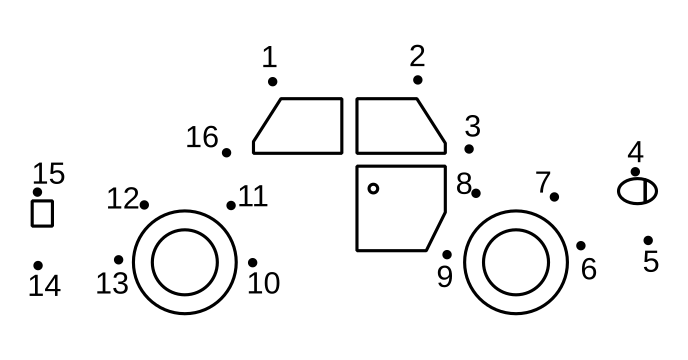
\includegraphics[width=.9\columnwidth]{images/carro.png}}
  \end{center}
  \begin{enumerate}
    \item Um carro.
    \item Uma moto.
    \item Um peixe.
    \item Um chocolate.
    \item Todas as anteriores.
  \end{enumerate}

  \item Qual dos seguinte \textbf{não é} um país?
  \begin{enumerate}
    \item Brasil.
    \item Inglaterra.
    \item Japão.
    \item Índia.
    \item África.
  \end{enumerate}

  \item Qual é a solução da equação a seguir?
  \[x^2 - 12x + 35x = 0\]
  \begin{enumerate}
    \item $x = 0$.
    \item $x = 7$.
    \item $x = 5$.
    \item $x = 10$.
    \item Estão corretas (b) e (c).
  \end{enumerate}

  \item Qual \textbf{não} é um dos quatro elementos?
  \begin{enumerate}
    \item Água.
    \item Terra.
    \item Fogo.
    \item Chocolate.
    \item Todos são os quatro elementos.
  \end{enumerate}

  \item \label{q:frutas}Se João tinha 4 laranjas e comeu uma delas, quantas laranjas ele tem agora?
  \begin{enumerate}
    \item 4 laranjas.
    \item 5 laranjas.
    \item 3 laranjas.
    \item 4 goiabas.
    \item Nenhuma laranja.
  \end{enumerate}

  \item Com relação a questão \ref{q:frutas}, o que João tinha que está sendo contado?
  \begin{enumerate}
    \item Frutas.
    \item Animais.
    \item Minerais.
    \item Gases.
    \item Nenhuma das alternativas.
  \end{enumerate}

  \item Qual dos seguinte \textbf{não é} um país?
  \begin{enumerate}
    \item Brasil.
    \item Inglaterra.
    \item Japão.
    \item Índia.
    \item África.
  \end{enumerate}

  \item Qual é a solução da equação a seguir?
  \[x^2 - 12x + 35x = 0\]
  \begin{enumerate}
    \item $x = 0$.
    \item $x = 7$.
    \item $x = 5$.
    \item $x = 10$.
    \item Estão corretas (b) e (c).
  \end{enumerate}

  \item Observe o código a seguir.
  \begin{snippet}
for (int i = 0; i < 10; i++) {
  printf("%d\n", i);
}
\end{snippet}
  O que ele faz?
  \begin{enumerate}
    \item Nada.
    \item Soma dois números.
    \item Subtrai dois números.
    \item Imprime o número 10 na tela.
    \item Imprime os números de 0 a 9 na tela.
  \end{enumerate}
\end{questoes}
\end{multicols}
\section{Responda às questões abaixo}
\centering(0,5 pts cada)
\begin{questoes}
  \item Nas linhas a seguir, discurse sobre a vida, o universo e tudo o mais.
  \pauta{4}
  \item Escreva com suas palavras o que é um ornitorrinco:
  \pauta{3}
\end{questoes}

\end{document}